\begin{figure}[h]
    \centering
    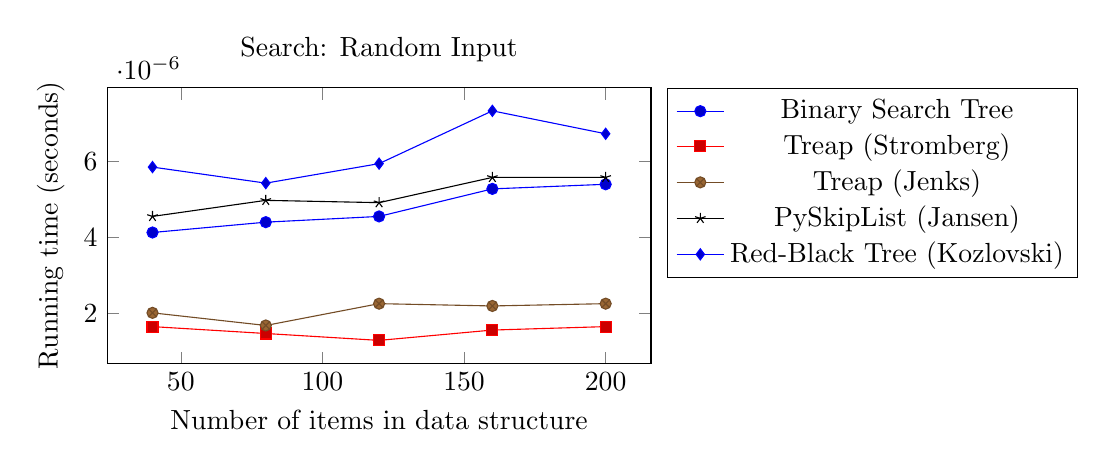
\begin{tikzpicture}
        \begin{axis}[
            xlabel={Number of items in data structure},
            ylabel={Running time (seconds)},
            title={Search: Random Input},
            width=0.7\textwidth,
            height=2in,
            legend pos=outer north east
        ]
		\addplot coordinates {
			(40, 4.126102113498342e-06)
			(80, 4.3971599165734674e-06)
			(120, 4.547747584950079e-06)
			(160, 5.270568393153652e-06)
			(200, 5.391038527854941e-06)
		};
		\addplot coordinates {
			(40, 1.6564643521330136e-06)
			(80, 1.4757591500838552e-06)
			(120, 1.2950539480319212e-06)
			(160, 1.5661117511084343e-06)
			(200, 1.6564643521344013e-06)
		};
		\addplot coordinates {
			(40, 2.0178747562368813e-06)
			(80, 1.686581885808336e-06)
			(120, 2.2588150256380725e-06)
			(160, 2.19857995828604e-06)
			(200, 2.2588150256366847e-06)
		};
		\addplot coordinates {
			(40, 4.547747584950079e-06)
			(80, 4.969393056403204e-06)
			(120, 4.9091579890525596e-06)
			(160, 5.571743729905488e-06)
			(200, 5.571743729905488e-06)
		};
		\addplot coordinates {
			(40, 5.842801532982e-06)
			(80, 5.421156061530263e-06)
			(120, 5.933154134007967e-06)
			(160, 7.3185606830658554e-06)
			(200, 6.716210009562185e-06)
		};
        \legend{Binary Search Tree, Treap (Stromberg), Treap (Jenks), PySkipList (Jansen), Red-Black Tree (Kozlovski)}
        \end{axis}
    \end{tikzpicture}
    \caption{Average of 10 operations, benchmarked every 40, starting at 40.}
\end{figure}